% Options for packages loaded elsewhere
\PassOptionsToPackage{unicode}{hyperref}
\PassOptionsToPackage{hyphens}{url}
\documentclass[
  10pt,
  a4paper,
]{article}
\usepackage{xcolor}
\usepackage[margin=1in]{geometry}
\usepackage{amsmath,amssymb}
\setcounter{secnumdepth}{-\maxdimen} % remove section numbering
\usepackage{iftex}
\ifPDFTeX
  \usepackage[T1]{fontenc}
  \usepackage[utf8]{inputenc}
  \usepackage{textcomp} % provide euro and other symbols
\else % if luatex or xetex
  \usepackage{unicode-math} % this also loads fontspec
  \defaultfontfeatures{Scale=MatchLowercase}
  \defaultfontfeatures[\rmfamily]{Ligatures=TeX,Scale=1}
\fi
\usepackage{lmodern}
\ifPDFTeX\else
  % xetex/luatex font selection
\fi
% Use upquote if available, for straight quotes in verbatim environments
\IfFileExists{upquote.sty}{\usepackage{upquote}}{}
\IfFileExists{microtype.sty}{% use microtype if available
  \usepackage[]{microtype}
  \UseMicrotypeSet[protrusion]{basicmath} % disable protrusion for tt fonts
}{}
\makeatletter
\@ifundefined{KOMAClassName}{% if non-KOMA class
  \IfFileExists{parskip.sty}{%
    \usepackage{parskip}
  }{% else
    \setlength{\parindent}{0pt}
    \setlength{\parskip}{6pt plus 2pt minus 1pt}}
}{% if KOMA class
  \KOMAoptions{parskip=half}}
\makeatother
\usepackage{color}
\usepackage{fancyvrb}
\newcommand{\VerbBar}{|}
\newcommand{\VERB}{\Verb[commandchars=\\\{\}]}
\DefineVerbatimEnvironment{Highlighting}{Verbatim}{commandchars=\\\{\}}
% Add ',fontsize=\small' for more characters per line
\newenvironment{Shaded}{}{}
\newcommand{\AlertTok}[1]{\textcolor[rgb]{1.00,0.00,0.00}{\textbf{#1}}}
\newcommand{\AnnotationTok}[1]{\textcolor[rgb]{0.38,0.63,0.69}{\textbf{\textit{#1}}}}
\newcommand{\AttributeTok}[1]{\textcolor[rgb]{0.49,0.56,0.16}{#1}}
\newcommand{\BaseNTok}[1]{\textcolor[rgb]{0.25,0.63,0.44}{#1}}
\newcommand{\BuiltInTok}[1]{\textcolor[rgb]{0.00,0.50,0.00}{#1}}
\newcommand{\CharTok}[1]{\textcolor[rgb]{0.25,0.44,0.63}{#1}}
\newcommand{\CommentTok}[1]{\textcolor[rgb]{0.38,0.63,0.69}{\textit{#1}}}
\newcommand{\CommentVarTok}[1]{\textcolor[rgb]{0.38,0.63,0.69}{\textbf{\textit{#1}}}}
\newcommand{\ConstantTok}[1]{\textcolor[rgb]{0.53,0.00,0.00}{#1}}
\newcommand{\ControlFlowTok}[1]{\textcolor[rgb]{0.00,0.44,0.13}{\textbf{#1}}}
\newcommand{\DataTypeTok}[1]{\textcolor[rgb]{0.56,0.13,0.00}{#1}}
\newcommand{\DecValTok}[1]{\textcolor[rgb]{0.25,0.63,0.44}{#1}}
\newcommand{\DocumentationTok}[1]{\textcolor[rgb]{0.73,0.13,0.13}{\textit{#1}}}
\newcommand{\ErrorTok}[1]{\textcolor[rgb]{1.00,0.00,0.00}{\textbf{#1}}}
\newcommand{\ExtensionTok}[1]{#1}
\newcommand{\FloatTok}[1]{\textcolor[rgb]{0.25,0.63,0.44}{#1}}
\newcommand{\FunctionTok}[1]{\textcolor[rgb]{0.02,0.16,0.49}{#1}}
\newcommand{\ImportTok}[1]{\textcolor[rgb]{0.00,0.50,0.00}{\textbf{#1}}}
\newcommand{\InformationTok}[1]{\textcolor[rgb]{0.38,0.63,0.69}{\textbf{\textit{#1}}}}
\newcommand{\KeywordTok}[1]{\textcolor[rgb]{0.00,0.44,0.13}{\textbf{#1}}}
\newcommand{\NormalTok}[1]{#1}
\newcommand{\OperatorTok}[1]{\textcolor[rgb]{0.40,0.40,0.40}{#1}}
\newcommand{\OtherTok}[1]{\textcolor[rgb]{0.00,0.44,0.13}{#1}}
\newcommand{\PreprocessorTok}[1]{\textcolor[rgb]{0.74,0.48,0.00}{#1}}
\newcommand{\RegionMarkerTok}[1]{#1}
\newcommand{\SpecialCharTok}[1]{\textcolor[rgb]{0.25,0.44,0.63}{#1}}
\newcommand{\SpecialStringTok}[1]{\textcolor[rgb]{0.73,0.40,0.53}{#1}}
\newcommand{\StringTok}[1]{\textcolor[rgb]{0.25,0.44,0.63}{#1}}
\newcommand{\VariableTok}[1]{\textcolor[rgb]{0.10,0.09,0.49}{#1}}
\newcommand{\VerbatimStringTok}[1]{\textcolor[rgb]{0.25,0.44,0.63}{#1}}
\newcommand{\WarningTok}[1]{\textcolor[rgb]{0.38,0.63,0.69}{\textbf{\textit{#1}}}}
\usepackage{longtable,booktabs,array}
\newcounter{none} % for unnumbered tables
\usepackage{calc} % for calculating minipage widths
% Correct order of tables after \paragraph or \subparagraph
\usepackage{etoolbox}
\makeatletter
\patchcmd\longtable{\par}{\if@noskipsec\mbox{}\fi\par}{}{}
\makeatother
% Allow footnotes in longtable head/foot
\IfFileExists{footnotehyper.sty}{\usepackage{footnotehyper}}{\usepackage{footnote}}
\makesavenoteenv{longtable}
\usepackage{graphicx}
\makeatletter
\newsavebox\pandoc@box
\newcommand*\pandocbounded[1]{% scales image to fit in text height/width
  \sbox\pandoc@box{#1}%
  \Gscale@div\@tempa{\textheight}{\dimexpr\ht\pandoc@box+\dp\pandoc@box\relax}%
  \Gscale@div\@tempb{\linewidth}{\wd\pandoc@box}%
  \ifdim\@tempb\p@<\@tempa\p@\let\@tempa\@tempb\fi% select the smaller of both
  \ifdim\@tempa\p@<\p@\scalebox{\@tempa}{\usebox\pandoc@box}%
  \else\usebox{\pandoc@box}%
  \fi%
}
% Set default figure placement to htbp
\def\fps@figure{htbp}
\makeatother
\setlength{\emergencystretch}{3em} % prevent overfull lines
\providecommand{\tightlist}{%
  \setlength{\itemsep}{0pt}\setlength{\parskip}{0pt}}
\usepackage{bookmark}
\IfFileExists{xurl.sty}{\usepackage{xurl}}{} % add URL line breaks if available
\urlstyle{same}
\hypersetup{
  pdftitle={EE6483 Mini Project: Literature Review and Comparative Experiments},
  pdfauthor={Section 1: Literature and Experiments},
  hidelinks,
  pdfcreator={LaTeX via pandoc}}

\title{EE6483 Mini Project: Literature Review and Comparative
Experiments}
\author{Section 1: Literature and Experiments}
\date{2 November 2026: revised experimental draft}

\begin{document}
\maketitle

\begin{quote}
\textbf{Status:} All five comparative experiments reported here have
been completed and checked against saved validation predictions. They
are single-seed results, not averages across multiple runs. The broader
screening of dozens of papers and systematic in-depth review of one or
two research groups remain to be completed. This section does not
replace the main-model, CIFAR-10 or class-imbalance sections of the
group report.
\end{quote}

\section{Abstract}\label{abstract}

We study which practical choices most affect validation accuracy in a
supervised Dogs vs.~Cats classifier. After excluding six redundant
training files, including one duplicate shared with validation, five
pipelines were evaluated on the same 19,994 training and 5,000
validation images. An ImageNet-pretrained ResNet18 with full
fine-tuning, mild augmentation and 224-pixel inputs reached 99.16\%
validation accuracy. Removing augmentation yielded 99.18\%, random
initialization yielded 93.28\%, reducing input resolution to 128 yielded
98.58\%, and a HOG--linear-SVM reference yielded 72.80\%. Among the
three controlled contrasts, pretrained initialization produced the
largest observed difference: 5.88 percentage points under the common
20-epoch budget. These results support pretrained fine-tuning as a
practical baseline for this dataset, while a one-image augmentation
difference, a single random seed and validation-based checkpoint
selection limit broader conclusions.

\section{1. Problem definition and
challenges}\label{problem-definition-and-challenges}

Image classification maps an image \(x\) to a label \(y\) from a
predefined label space. For Dogs vs.~Cats, the task is supervised binary
classification with \(\mathcal{Y}=\{\text{cat},\text{dog}\}\). The
prediction is \(\hat{y}=\arg\max_{y\in\mathcal{Y}}p(y\mid x)\); the
submission uses 0 for cat and 1 for dog. The provided training and
validation sets have labels, whereas the 500 test images require
predictions {[}1{]}.

Key challenges include intra-class variation among breeds, similar
appearance across classes, pose and scale changes, occlusion, image
quality, background shortcuts, limited labelled data and possible
distribution shift. A high validation accuracy does not by itself
establish robustness to unknown classes or unseen domains.

\section{2. Learning settings}\label{learning-settings}

\subsection{2.1 Supervised versus unsupervised and self-supervised
learning}\label{supervised-versus-unsupervised-and-self-supervised-learning}

Supervised learning uses labelled pairs \((x_i,y_i)\) and optimizes an
objective such as cross-entropy. The project has labelled cat and dog
images and can therefore train a supervised classifier directly. Its
limitations include reliance on labels and the possibility of
overfitting.

Unsupervised learning instead searches for structure without human
category labels; clustering need not recover cat and dog classes.
Self-supervised learning constructs a training signal from data itself
to learn transferable features. SimCLR contrasts two augmented views of
an image {[}3{]}; MAE reconstructs masked image patches {[}4{]}; DINOv2
learns general-purpose visual features without supervised class labels
{[}5{]}. Self-supervised pretraining can be followed by supervised
training on the target labels: an unlabeled pretraining stage does not
imply that downstream classification is label-free. Large-scale
pretraining also incurs external data and compute costs.

\subsection{2.2 Closed-set versus open-set
recognition}\label{closed-set-versus-open-set-recognition}

Closed-set classification assumes test classes belong to the known
training label set. This project requires every test prediction to be
cat or dog, so its stated protocol is closed-set binary classification.
Open-set recognition additionally requires the system to identify inputs
from unknown classes, for example a rabbit, rather than force them into
a known class {[}6{]}. A two-class softmax classifier cannot by itself
guarantee reliable unknown-class detection; open-set performance
requires a separate evaluation with unknown examples. We discuss this
setting but do not claim to implement it.

\subsection{2.3 Distribution shift}\label{distribution-shift}

Distribution shift occurs when the source and target distributions
differ, for instance in lighting, camera, backgrounds or animal breeds.
Domain adaptation uses information from a target domain during
development, whereas domain generalization seeks performance on unseen
domains without using their data during training. The exact permitted
target information depends on the adaptation setting. Transfer learning
and augmentation are plausible tools for improved generalization, but
neither guarantees robustness. Because the project does not prescribe a
separate target-domain evaluation, performance on its validation set
must not be presented as proof of out-of-domain generalization.

\section{3. Representative work and baseline
selection}\label{representative-work-and-baseline-selection}

ResNet learns residual functions through skip connections, \(y=F(x)+x\),
facilitating the optimization of deeper convolutional networks {[}2{]}.
ConvNeXt revisits the design and training of convolutional networks in
the context of modern vision architectures {[}8{]}. These works motivate
studying architectural choices together with training practices, rather
than assuming one architecture is universally best.

SimCLR {[}3{]}, MAE {[}4{]}, and DINOv2 {[}5{]} illustrate different
routes to transferable representations: contrastive view matching,
masked reconstruction, and self-supervised visual feature learning.
These methods show why pretraining can help, but their reported
benchmark results do not establish their ranking on this project's
dataset.

We adopt ImageNet-pretrained ResNet18 with a newly initialized
two-output linear head as the baseline. A labelled binary task permits
direct supervised fine-tuning, while reusing a pretrained representation
avoids learning every feature from random initialization. ResNet18 also
permits several controlled runs on the available 6 GB laptop GPU.
Research on feature transfer shows that transferability depends on layer
specificity and source--target similarity, and that benefits can persist
after fine-tuning {[}7{]}. This motivates testing transfer, rather than
assuming it must help.

Our completed E1--E3 comparison supports this choice under the actual
training budget: pretrained full fine-tuning achieved 99.16\%, compared
with 93.28\% from random initialization. The required adaptation was to
replace the original classification head, normalize inputs consistently
with the pretrained model and optimize all layers on the target labels.
This does not establish that full fine-tuning outperforms freezing the
backbone: a frozen-feature configuration was not run. ImageNet
pretraining also adds external data and computation; possible overlap
with the target data was not audited. The baseline rationale therefore
combines practical suitability with a measured, budget-specific
advantage, rather than a claim of universal superiority.

\textbf{Further literature work required:} Build an auditable screening
table covering dozens of relevant papers, document search queries and
selection criteria, and carry out in-depth reading of one or two
research groups. Candidate research lines are ResNet/ConvNeXt and
DINO/DINOv2; these are proposed starting points, not a completed team
survey. Check original papers and author affiliations before making
claims about teams or current rankings.

\section{4. Comparative experimental
method}\label{comparative-experimental-method}

\subsection{4.1 Data audit and leakage
control}\label{data-audit-and-leakage-control}

The teacher-provided archive contained 20,000 training images (10,000
per class), 5,000 validation images (2,500 per class) and 500 unlabelled
test images. All 25,500 images decoded successfully as RGB. We retained
the supplied split rather than randomly repartitioning the data. The
mapping was explicitly fixed as cat = 0 and dog = 1.

SHA-256 file hashes revealed five groups of exact duplicates. One group
contained a training image and a validation image; the other groups were
entirely within training. We retained every validation image, excluded
the training-side copy of the cross-split duplicate, and removed
redundant training-only copies. Six training paths were excluded in
total, leaving \textbf{19,994 training images: 9,997 cats and 9,997
dogs}. Every experiment used these same training paths and all 5,000
validation paths. Original files were preserved; exclusions were applied
through a shared manifest. This removes the detected exact-duplicate
leakage, but byte hashes cannot rule out re-encoded or perceptually
similar images. Model development did not use the 500 test images.

\subsection{4.2 Neural preprocessing and
optimization}\label{neural-preprocessing-and-optimization}

For output size \(s\), the shorter image side was resized to
\(\operatorname{round}(256s/224)\) while preserving aspect ratio,
followed by an \(s \times s\) centre crop. Thus the resize/crop sizes
were 256/224 for E1--E3 and 146/128 for E4. In augmented runs, a random
horizontal flip (probability 0.5) and rotation sampled uniformly from
\([-10^\circ,10^\circ]\) followed the crop. Validation used resize and
crop only. Tensors were normalized channel-wise with ImageNet mean
\((0.485,0.456,0.406)\) and standard deviation \((0.229,0.224,0.225)\).

E1--E4 used ResNet18 with a two-output linear layer in place of its
original classification head. E1, E2 and E4 loaded torchvision's
\texttt{ResNet18\_Weights.IMAGENET1K\_V1}; E3 used random
initialization. The pretrained weights came from supervised ImageNet
training; the self-supervised methods discussed in the review were not
implemented here. All parameters were trainable: no backbone freezing
was applied. For an input batch of size \(B\), the network accepted
\(B \times 3 \times s \times s\) and returned \(B \times 2\) logits.
Cross-entropy was applied directly to the logits; predictions were their
argmax.

{\def\LTcaptype{none} % do not increment counter
\begin{longtable}[]{@{}
  >{\raggedright\arraybackslash}p{(\linewidth - 2\tabcolsep) * \real{0.5000}}
  >{\raggedright\arraybackslash}p{(\linewidth - 2\tabcolsep) * \real{0.5000}}@{}}
\toprule\noalign{}
\begin{minipage}[b]{\linewidth}\raggedright
Setting
\end{minipage} & \begin{minipage}[b]{\linewidth}\raggedright
Implemented value
\end{minipage} \\
\midrule\noalign{}
\endhead
\bottomrule\noalign{}
\endlastfoot
Epochs / batch size & 20 / 16, for every neural configuration \\
Optimizer & SGD, momentum 0.9, weight decay \(10^{-4}\) \\
Initial learning rate & 0.001, common to E1--E4; no separate
learning-rate search \\
Schedule & CosineAnnealingLR, \(T_{\max}=20\), default minimum learning
rate 0 \\
Precision & CUDA automatic mixed precision with gradient scaling \\
Random seed & 42 for Python, NumPy and PyTorch \\
Data loading & Two workers; training shuffled, validation unshuffled \\
Checkpoint selection & Highest validation accuracy across 20 epochs;
earliest epoch on ties \\
Hardware / framework & NVIDIA RTX 3060 Laptop GPU, 6 GB; PyTorch
2.5.1+cu121; torchvision 0.20.1+cu121 \\
\end{longtable}
}

The code disabled cuDNN benchmarking and enabled deterministic cuDNN
behavior. These measures document the attempt to control randomness;
they do not guarantee bitwise agreement on every software/hardware
combination. Each configuration was run once, so we do not report a
cross-seed mean, standard deviation or confidence interval.

\subsection{4.3 Five configurations and interpretation of
controls}\label{five-configurations-and-interpretation-of-controls}

{\def\LTcaptype{none} % do not increment counter
\begin{longtable}[]{@{}
  >{\raggedright\arraybackslash}p{(\linewidth - 8\tabcolsep) * \real{0.2000}}
  >{\raggedright\arraybackslash}p{(\linewidth - 8\tabcolsep) * \real{0.2000}}
  >{\raggedright\arraybackslash}p{(\linewidth - 8\tabcolsep) * \real{0.2000}}
  >{\raggedright\arraybackslash}p{(\linewidth - 8\tabcolsep) * \real{0.2000}}
  >{\raggedright\arraybackslash}p{(\linewidth - 8\tabcolsep) * \real{0.2000}}@{}}
\toprule\noalign{}
\begin{minipage}[b]{\linewidth}\raggedright
ID
\end{minipage} & \begin{minipage}[b]{\linewidth}\raggedright
Pipeline
\end{minipage} & \begin{minipage}[b]{\linewidth}\raggedright
Initialization
\end{minipage} & \begin{minipage}[b]{\linewidth}\raggedright
Random augmentation
\end{minipage} & \begin{minipage}[b]{\linewidth}\raggedright
Input
\end{minipage} \\
\midrule\noalign{}
\endhead
\bottomrule\noalign{}
\endlastfoot
E1 & ResNet18, full fine-tuning & ImageNet V1 & Flip + rotation & RGB,
224 \\
E2 & ResNet18, full fine-tuning & ImageNet V1 & None & RGB, 224 \\
E3 & ResNet18, trained from scratch & Random & Flip + rotation & RGB,
224 \\
E4 & ResNet18, full fine-tuning & ImageNet V1 & Flip + rotation & RGB,
128 \\
E5 & HOG + standardization + linear SVM & No neural pretraining & None &
Grayscale, 128 \\
\end{longtable}
}

E1 versus E2 evaluates the chosen augmentation policy; E1 versus E3
evaluates initialization under a common optimization recipe; E1 versus
E4 evaluates input resolution. The data lists, architecture, epoch
count, batch size, loss, optimizer, schedule and selection rule were
held fixed across the relevant neural contrasts. Equal epochs do not
imply equal runtime or equally well-tuned optimization. In particular, a
randomly initialized network may benefit from another learning rate or
longer training, neither of which was tested here.

For E5, images were converted to grayscale and resized directly to
\(128 \times 128\). HOG used nine orientations, \(16 \times 16\) pixels
per cell and \(2 \times 2\) cells per block, producing 1,764 features.
The HOG descriptor {[}9{]} was combined with a linear support-vector
classifier {[}10{]}. StandardScaler was fitted on training features only
and then applied to validation features. LinearSVC used \(C=1\),
\texttt{max\_iter=10000} and seed 42; no SVM hyperparameter search was
performed. E5 used the full cleaned training set. As color, feature
learning, geometry handling and classifier all change, E5 is a
pipeline-level reference rather than an isolated test of the classifier.

\section{5. Results and discussion}\label{results-and-discussion}

\subsection{5.1 Validation performance}\label{validation-performance}

All neural results below come from the selected best checkpoint, not
necessarily the final epoch. Per-class recall is the proportion of true
members of a class correctly classified; the two classes each contain
2,500 validation images.

{\def\LTcaptype{none} % do not increment counter
\begin{longtable}[]{@{}
  >{\raggedright\arraybackslash}p{(\linewidth - 10\tabcolsep) * \real{0.1304}}
  >{\raggedleft\arraybackslash}p{(\linewidth - 10\tabcolsep) * \real{0.1739}}
  >{\raggedleft\arraybackslash}p{(\linewidth - 10\tabcolsep) * \real{0.1739}}
  >{\raggedleft\arraybackslash}p{(\linewidth - 10\tabcolsep) * \real{0.1739}}
  >{\raggedleft\arraybackslash}p{(\linewidth - 10\tabcolsep) * \real{0.1739}}
  >{\raggedleft\arraybackslash}p{(\linewidth - 10\tabcolsep) * \real{0.1739}}@{}}
\toprule\noalign{}
\begin{minipage}[b]{\linewidth}\raggedright
ID
\end{minipage} & \begin{minipage}[b]{\linewidth}\raggedleft
Accuracy
\end{minipage} & \begin{minipage}[b]{\linewidth}\raggedleft
Cat recall
\end{minipage} & \begin{minipage}[b]{\linewidth}\raggedleft
Dog recall
\end{minipage} & \begin{minipage}[b]{\linewidth}\raggedleft
Errors / 5,000
\end{minipage} & \begin{minipage}[b]{\linewidth}\raggedleft
Best epoch
\end{minipage} \\
\midrule\noalign{}
\endhead
\bottomrule\noalign{}
\endlastfoot
E1 & 99.16\% & 98.72\% & 99.60\% & 42 & 18 \\
E2 & 99.18\% & 99.32\% & 99.04\% & 41 & 6 \\
E3 & 93.28\% & 93.88\% & 92.68\% & 336 & 18 \\
E4 & 98.58\% & 98.36\% & 98.80\% & 71 & 17 \\
E5 & 72.80\% & 72.36\% & 73.24\% & 1,360 & N/A \\
\end{longtable}
}

E1's confusion matrix, with rows denoting true classes and columns
predicted classes in the order cat, dog, was

\[
C_{\mathrm{E1}}=\begin{pmatrix}2468&32\\10&2490\end{pmatrix}.
\]

Thus 32 cats were predicted as dogs and 10 dogs as cats. E2's
corresponding counts were 17 and 24: its slightly higher aggregate
accuracy did not improve both class recalls. These counts identify what
changed in the validation outcomes; they do not establish visual causes
of individual mistakes without inspecting the images.

\begin{figure}
\centering
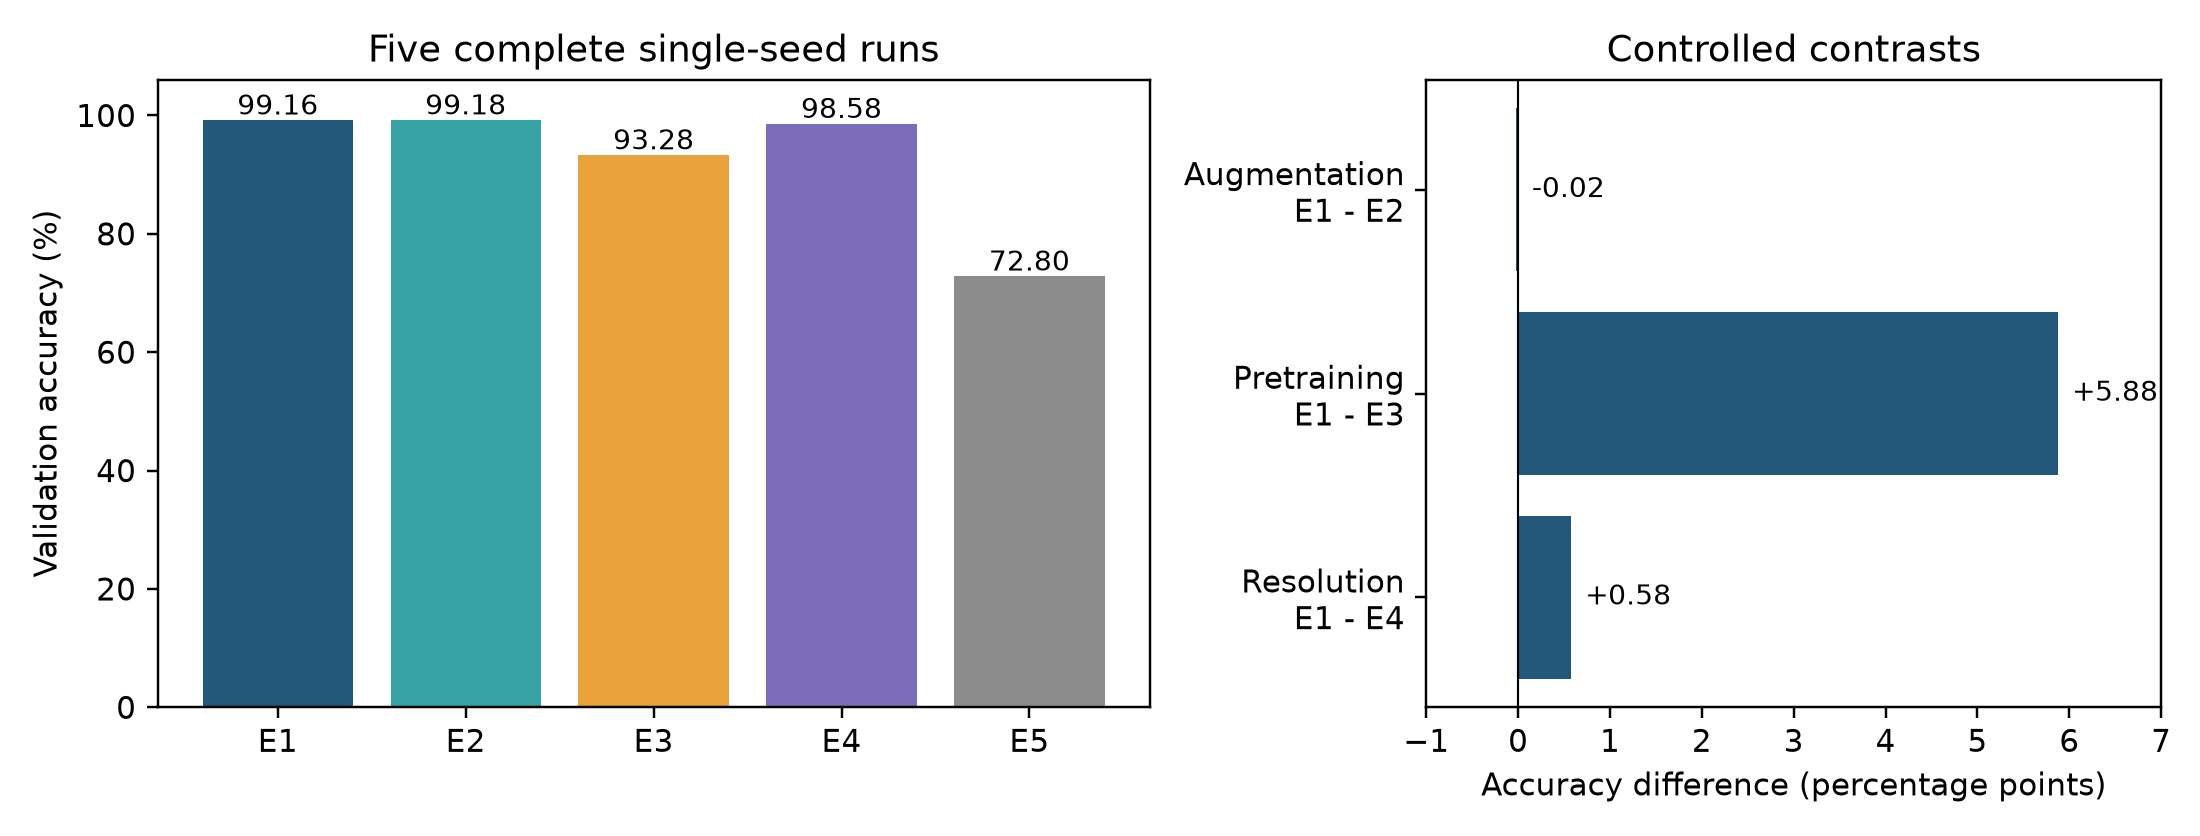
\includegraphics[width=0.95\linewidth,height=\textheight,keepaspectratio,alt={Validation accuracy for all five completed configurations. Every bar represents one run with seed 42; no error bars are inferred from a single run.}]{figures/validation_accuracy.png}
\caption{Validation accuracy for all five completed configurations.
Every bar represents one run with seed 42; no error bars are inferred
from a single run.}
\end{figure}

\subsection{5.2 Which factor had the largest observed
effect?}\label{which-factor-had-the-largest-observed-effect}

We define a signed contrast as E1 accuracy minus the comparison
accuracy, expressed in percentage points (pp). A positive difference
favors E1. With 5,000 validation images, one additional correct
prediction changes accuracy by 0.02 pp.

{\def\LTcaptype{none} % do not increment counter
\begin{longtable}[]{@{}
  >{\raggedright\arraybackslash}p{(\linewidth - 6\tabcolsep) * \real{0.2143}}
  >{\raggedright\arraybackslash}p{(\linewidth - 6\tabcolsep) * \real{0.2143}}
  >{\raggedleft\arraybackslash}p{(\linewidth - 6\tabcolsep) * \real{0.2857}}
  >{\raggedleft\arraybackslash}p{(\linewidth - 6\tabcolsep) * \real{0.2857}}@{}}
\toprule\noalign{}
\begin{minipage}[b]{\linewidth}\raggedright
Contrast
\end{minipage} & \begin{minipage}[b]{\linewidth}\raggedright
Factor
\end{minipage} & \begin{minipage}[b]{\linewidth}\raggedleft
Difference (pp)
\end{minipage} & \begin{minipage}[b]{\linewidth}\raggedleft
E1 advantage in correct predictions
\end{minipage} \\
\midrule\noalign{}
\endhead
\bottomrule\noalign{}
\endlastfoot
E1 minus E2 & Chosen augmentation & -0.02 & -1 \\
E1 minus E3 & Pretrained initialization & +5.88 & +294 \\
E1 minus E4 & 224 rather than 128 input & +0.58 & +29 \\
\end{longtable}
}

\textbf{Pretrained initialization had the largest observed effect among
these three contrasts.} Holding the specified architecture and training
recipe fixed, it reduced errors from 336 to 42. This supports starting
from pretrained features when training time and hardware are limited.
The difference includes the advantage of external ImageNet training and
is conditional on the common 20-epoch schedule, not evidence that a
separately optimized scratch model could never match it.

\textbf{The chosen augmentation policy produced no measurable advantage
in this single-run comparison.} E2 exceeded E1 by just one correct
prediction. We therefore retain mild augmentation as a reasonable
baseline design choice, but do not claim that these results demonstrate
an accuracy benefit from it. Conversely, they do not justify rejecting
augmentation in general. Only horizontal flips plus mild rotations, one
seed and this validation split were tested; the two transforms were not
ablated separately. Paired seed values also do not force identical
stochastic training trajectories when transformation policies differ.
The small observed difference should be checked across additional runs
before choosing a final augmentation policy.

\textbf{Higher input resolution improved accuracy modestly in this
setting.} E1 correctly classified 29 more images than E4. Preserving
finer image detail is a plausible explanation, but these experiments do
not identify which visual features caused the difference. E4 still
achieved 98.58\%, making lower resolution a candidate when resource
constraints matter. Choosing it requires a separate, controlled
measurement of speed and memory rather than assuming the observed
wall-clock ratio is an intrinsic speedup.

The HOG--SVM pipeline was 26.36 pp below E1, corresponding to 1,318 more
validation errors. This is consistent with pretrained, trainable
representations being useful here, but the comparison also changes color
information, preprocessing and classifier. It cannot isolate the benefit
of convolution, the SVM, or pretraining alone. An untuned HOG
configuration also does not establish an upper bound on traditional
methods.

\subsection{5.3 Learning dynamics and checkpoint
selection}\label{learning-dynamics-and-checkpoint-selection}

Pretraining gave a substantial early advantage: E1 reached 98.68\%
validation accuracy after one epoch, whereas E3 reached 69.64\%. E3
improved to 93.28\% by its best epoch, showing that training from
scratch learned the task, but did not catch up under this schedule.
These trajectories support a budget-specific interpretation of transfer
benefits rather than a claim that the scratch model was optimized to its
limit.

At E1's best epoch, training accuracy was 99.90\% and validation
accuracy 99.16\%. Near-perfect training performance therefore did not
remove validation errors. E2 peaked at epoch 6 (99.18\%) and ended at
98.98\%, illustrating why using the final epoch would change the
comparison. E1 also ended below its peak, at 99.06\%. Such fluctuations
and train--validation gaps motivate validation-based checkpoint
selection, but do not by themselves prove a particular cause of
overfitting. Training accuracy is measured online during optimization
and, in augmented runs, on transformed images, so it is not the same as
a separate deterministic training-set evaluation.

\begin{figure}
\centering
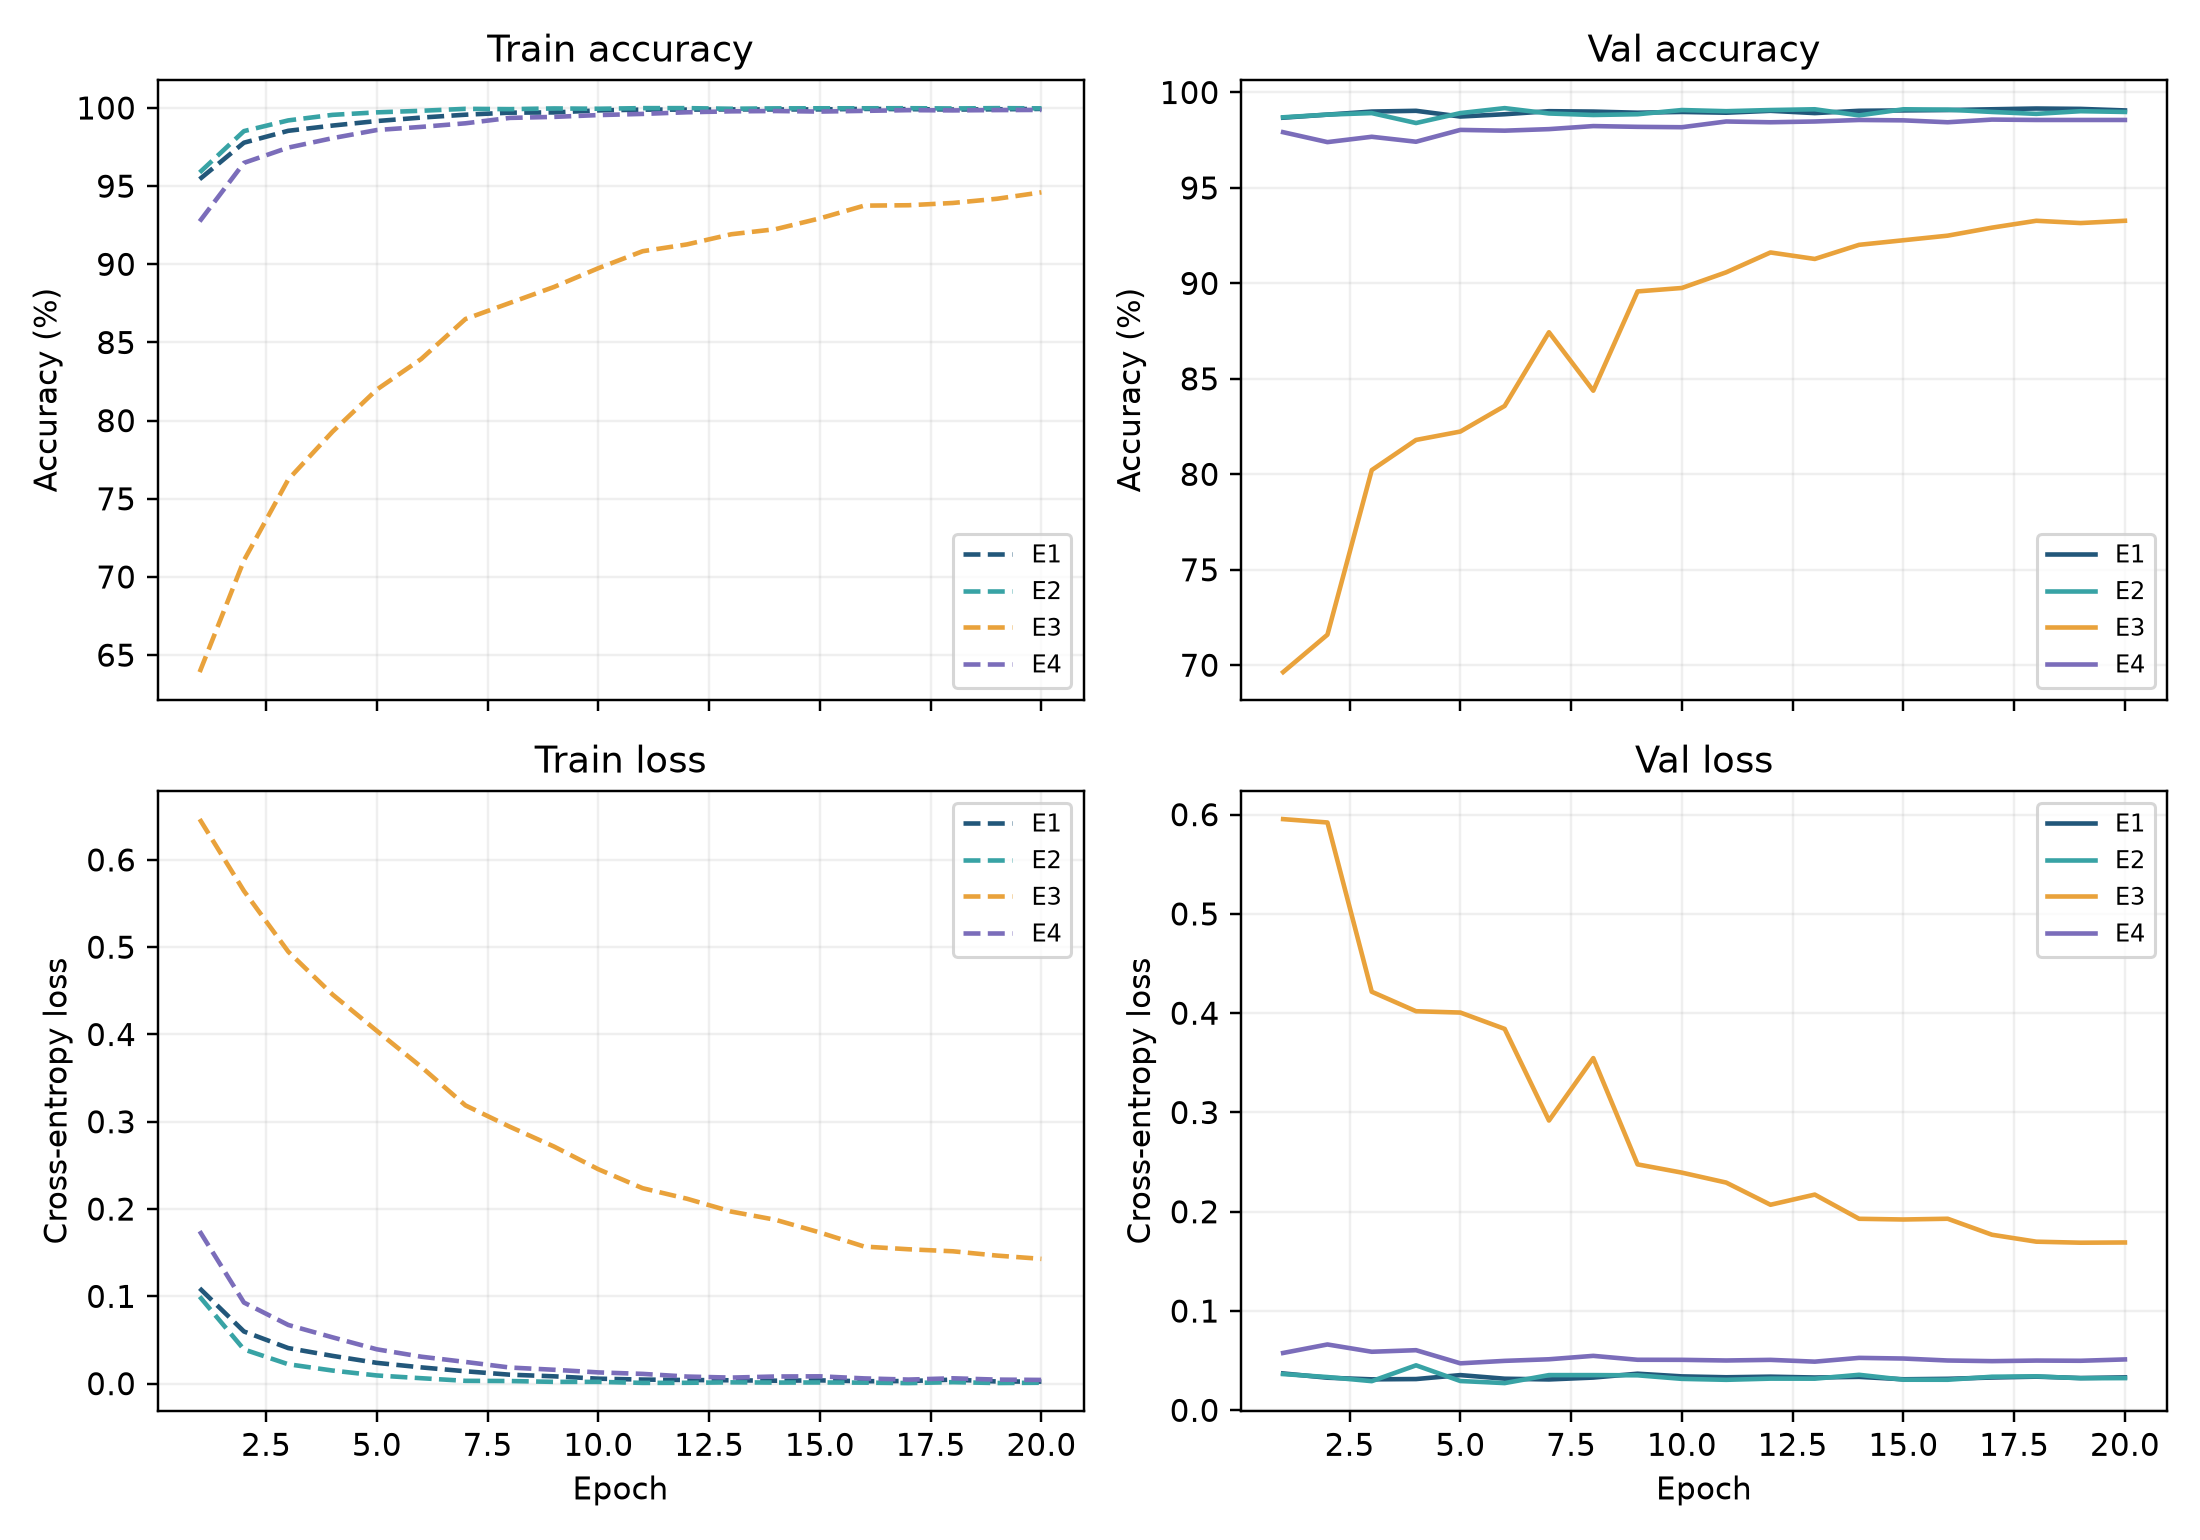
\includegraphics[width=0.98\linewidth,height=\textheight,keepaspectratio,alt={Training and validation accuracy and loss across all 20 epochs. Dashed lines denote training measurements; solid lines denote validation measurements. These are single-run learning curves.}]{figures/learning_curves.png}
\caption{Training and validation accuracy and loss across all 20 epochs.
Dashed lines denote training measurements; solid lines denote validation
measurements. These are single-run learning curves.}
\end{figure}

\subsection{5.4 Runtime and resource
interpretation}\label{runtime-and-resource-interpretation}

{\def\LTcaptype{none} % do not increment counter
\begin{longtable}[]{@{}lrr@{}}
\toprule\noalign{}
ID & Recorded end-to-end time (s) & Time (min) \\
\midrule\noalign{}
\endhead
\bottomrule\noalign{}
\endlastfoot
E1 & 1,731.0 & 28.85 \\
E2 & 1,119.8 & 18.66 \\
E3 & 1,070.7 & 17.85 \\
E4 & 748.0 & 12.47 \\
E5 & 291.5 & 4.86 \\
\end{longtable}
}

These are observed pipeline times, not isolated training times. The
neural timer covers model construction, training, validation and
checkpoint/log saving; the SVM timer covers feature extraction, scaling,
fitting, prediction and model saving. Initial dataset enumeration and
manifest writing occur before the timer. The GPU was shared with other
activity, and E5 ran on CPU concurrently with part of E1. E1's first
three epochs took approximately 113--124 seconds each, while its last
epoch took about 58 seconds. Consequently, the total times are useful
execution records but not a fair benchmark of architectural speed or
augmentation overhead. Peak memory and controlled inference latency were
not recorded and are not claimed.

\subsection{5.5 Scope and limitations}\label{scope-and-limitations}

First, each configuration used seed 42 only. We cannot estimate
cross-run variability, claim statistical significance, or substitute
these results for the main-model owner's three-seed final evaluation.
Second, validation data selected the best checkpoint and informed the
comparisons; these accuracies may be optimistic estimates of performance
on unseen data. They are not test-set accuracies. Third, we controlled
the common recipe rather than tuning each pipeline independently, so the
results compare specific implementations under a shared budget. Fourth,
exact-byte deduplication does not establish that all near duplicates or
pretraining overlaps have been removed. Fifth, the separate effects of
individual augmentations, frozen versus unfrozen features, and
interactions among initialization, resolution and augmentation remain
untested. Finally, the experiments are closed-set and do not evaluate
unknown-class rejection or explicit domain shift.

\section{6. Reproducibility and integration into the group
report}\label{reproducibility-and-integration-into-the-group-report}

The implementation is in \path{section1/run_experiment.py}, with data
preparation in \path{section1/prepare_data.py} and the formal queue in
\path{section1/run_all.py}. The following commands assume that the
teacher-provided archive is saved as \path{data/datasets.zip} and are
run from the repository root:

\begin{Shaded}
\begin{Highlighting}[]
\ExtensionTok{conda}\NormalTok{ activate ee6483}
\ExtensionTok{python}\NormalTok{ section1/prepare\_data.py}
\ExtensionTok{python}\NormalTok{ section1/run\_all.py}
\ExtensionTok{python}\NormalTok{ section1/summarize\_results.py}
\end{Highlighting}
\end{Shaded}

The queue skips already completed runs. For a fresh independent
replication, use a separate output directory with
\texttt{run\_experiment.py}; do not overwrite the archived results. For
example:

\begin{Shaded}
\begin{Highlighting}[]
\ExtensionTok{python}\NormalTok{ section1/run\_experiment.py }\DataTypeTok{\textbackslash{}}
  \AttributeTok{{-}{-}data}\NormalTok{ data/datasets }\AttributeTok{{-}{-}experiment}\NormalTok{ E1 }\AttributeTok{{-}{-}epochs}\NormalTok{ 20 }\DataTypeTok{\textbackslash{}}
  \AttributeTok{{-}{-}seed}\NormalTok{ 42 }\AttributeTok{{-}{-}batch{-}size}\NormalTok{ 16 }\AttributeTok{{-}{-}workers}\NormalTok{ 2 }\AttributeTok{{-}{-}amp} \DataTypeTok{\textbackslash{}}
  \AttributeTok{{-}{-}exclude}\NormalTok{ section1/artifacts/excluded\_train.json }\DataTypeTok{\textbackslash{}}
  \AttributeTok{{-}{-}output}\NormalTok{ section1/results/replication}
\end{Highlighting}
\end{Shaded}

The audit and exclusion manifest are in \path{section1/artifacts/}.
Small configurations, metrics and training histories are copied to
\path{section1/artifacts/runs/}; the consolidated table is
\path{section1/artifacts/results.csv}. Original best weights, full
validation predictions and logs remain under
\path{section1/results/formal/}. Configurations record the experiment
source hash and weight version. Automated checks confirmed equal
training/validation file lists across E1--E5, 5,000 predictions per
configuration, agreement between saved predictions and reported
accuracy, and 20 epochs for each neural run.

Before merging this section into the group report, the main-model owner
should use the same six-file exclusion manifest or explicitly disclose a
different split. A frozen-backbone experiment, tuned final model,
three-seed statistics, test prediction CSV, CIFAR-10 and imbalance
analysis are outside the completed comparisons reported here. The
literature requirement also still needs a documented screening table
covering dozens of papers and detailed reading of one or two research
groups; the representative citations above are not presented as
completion of that requirement.

\section{References}\label{references}

{[}1{]} EE6483, \emph{Mini Project (Option 2): Dogs vs.~Cats},
assignment brief, 2026. Dataset and submission template supplied by the
teaching team.

{[}2{]} K. He, X. Zhang, S. Ren, and J. Sun, ``Deep Residual Learning
for Image Recognition,'' CVPR, 2016.
\url{https://openaccess.thecvf.com/content_cvpr_2016/html/He_Deep_Residual_Learning_CVPR_2016_paper.html}

{[}3{]} T. Chen, S. Kornblith, M. Norouzi, and G. Hinton, ``A Simple
Framework for Contrastive Learning of Visual Representations,'' ICML,
2020. \url{https://proceedings.mlr.press/v119/chen20j.html}

{[}4{]} K. He et al., ``Masked Autoencoders Are Scalable Vision
Learners,'' CVPR, 2022.
\url{https://openaccess.thecvf.com/content/CVPR2022/html/He_Masked_Autoencoders_Are_Scalable_Vision_Learners_CVPR_2022_paper.html}

{[}5{]} M. Oquab et al., ``DINOv2: Learning Robust Visual Features
without Supervision,'' 2023. \url{https://arxiv.org/abs/2304.07193}

{[}6{]} C. Geng, S.-J. Huang, and S. Chen, ``Recent Advances in Open Set
Recognition: A Survey,'' 2018. \url{https://arxiv.org/abs/1811.08581}

{[}7{]} J. Yosinski, J. Clune, Y. Bengio, and H. Lipson, ``How
transferable are features in deep neural networks?'' Advances in Neural
Information Processing Systems 27, 2014.
\url{https://proceedings.neurips.cc/paper_files/paper/2014/hash/532a2f85b6977104bc93f8580abbb330-Abstract.html}

{[}8{]} Z. Liu et al., ``A ConvNet for the 2020s,'' CVPR, 2022.
\url{https://openaccess.thecvf.com/content/CVPR2022/html/Liu_A_ConvNet_for_the_2020s_CVPR_2022_paper.html}

{[}9{]} N. Dalal and B. Triggs, ``Histograms of Oriented Gradients for
Human Detection,'' CVPR, 2005.
\url{https://lear.inrialpes.fr/people/triggs/pubs/Dalal-cvpr05.pdf}

{[}10{]} C. Cortes and V. Vapnik, ``Support-vector networks,'' Machine
Learning, vol.~20, pp.~273--297, 1995.
\url{https://doi.org/10.1007/BF00994018}

\end{document}
